\documentclass[brazilian,12pt,a4paper,final]{article}
\DeclareUnicodeCharacter{2219}{\textbullet}
\usepackage[brazilian]{babel}
\usepackage{nonfloat}
\usepackage[utf8]{inputenc}
\usepackage{multicol}
\usepackage{hyperref}
\usepackage[pdftex]{color,graphicx}
\usepackage{geometry}
\usepackage{amsmath}
\usepackage{dirtytalk}
 \geometry{
 a4paper,
 total={170mm,257mm},
 left=20mm,
 top=20mm,
 }
\usepackage{fancyhdr}
\usepackage{caption}[=v1]
\usepackage{xcolor}
\pagestyle{fancy}
\fancyhead{}
\lhead{
\includegraphics[width=1.5cm]{logoufrgs}}
\rhead{
\includegraphics[width=0.8cm]{logoif}}
\fancyfoot{}
\fancyhead[C]{\footnotesize Física Experimental II - A (FIS01260) \bullet 2024/2}
\fancyfoot[RO,LE]{\thepage}

\pagestyle{empty}
\title{Determinação Experimental do Calor Latente de Vaporização do Nitrogênio Líquido}
\author{Aluno: Pedro Henrique Reis de Oliveira - Matrícula: 00590908 \\ IF-UFRGS}
\date{Dezembro 2024}

\begin{document}
\maketitle
%\tableofcontents
\thispagestyle{fancy} 

\section*{Resumo}
\paragraph{}
Este relatório descreve um experimento realizado para determinar o calor latente de vaporização do nitrogênio líquido utilizando um método calorimétrico. O objetivo principal foi medir a energia necessária para a mudança de fase do nitrogênio líquido para vapor à pressão atmosférica, combinando medições da taxa de evaporação natural e induzida por uma fonte de calor conhecida. Foram realizadas medições de massa, tempo, corrente e tensão, e posteriormente o tratamento de dados.

\section{Introdução}
\paragraph{}

O calor latente é uma grandeza física essencial na termodinâmica, representando a quantidade de energia necessária para que uma substância mude de fase sem alteração de temperatura. Este fenômeno está presente em diversos processos do cotidiano, desde a evaporação da água durante o cozimento de alimentos até aplicações industriais como sistemas de refrigeração. No caso específico do nitrogênio líquido, seu baixo ponto de ebulição (aproximadamente 77K ou -196°C) e alto calor latente de vaporização o tornam ideal para diversas aplicações, desde a conservação de materiais biológicos até o resfriamento de supercondutores. Este experimento visa determinar experimentalmente o calor latente de vaporização do nitrogênio líquido à pressão atmosférica, utilizando um método calorimétrico que combina a medição da taxa de evaporação natural com aquela induzida por uma fonte de calor conhecida.

\section{Embasamento Teórico}
\label{embas}
Partimos da seguinte relação porque não temos variação da energia interna e trabalho desprezível realizado sobre/pelo o sistema:
$$
    Q = mL_v
$$
Para relacionar essas grandezas experimentalmente, analisaremos sua variação, portanto:
$$
    \frac{dQ}{dt} = \frac{d(mL_v)}{dt}
$$
\newpage
A energia transferida para o sistema vêm do resistor, mas também existe contribuição da energia fornecida pelo próprio ambiente ao sistema. Portanto, para os cálculos precisaremos considerar apenas a energia dada pelo resistor, fazemos:
$$
    \frac{dm_{total}}{dt} = \frac{dm_{aquecedor}}{dt} + \frac{dm_{ambiente}}{dt}
$$
Considerando que a potência fornecida pelo resistor é constante e equivalente a energia transferida via calor, temos:
$$
    P = \frac{dQ}{dt} = \frac{dm_{aquecedor}}{dt}L_v = i \cdot V
$$
Aproximando a variação da massa como:
$$
    \frac{dm_{aquecedor}}{dt} = \frac{m_{final} - m_{inicial}}{t_{final} - t_{inicial}}
$$
Podemos calcular o calor latente de vaporização como:
$$
    L_v = \frac{P}{\frac{m_{final} - m_{inicial}}{t_{final} - t_{inicial}}}
$$
Mais detalhes, demonstrações e cálculos completos podem ser encontrados no capítulo 18.8 do livro Fundamentos de Física, de Halliday e Resnick \cite{Halliday - 9 ed}.

\section{Materiais Utilizados}
\paragraph{}
Foram utilizados para o experimento os seguintes materiais e instrumentos:
\begin{enumerate}
    \item Amostra de nitrogênio líquido
    \item Balança analógica (Precisão 0,1g)
    \item Calorímetro
    \item Cronômetro (Precisão 0,01s)
    \item Resistor de potência
    \item Fonte de tensão contínua
    \item Dois multímetros digitais (Precisão 0,001V e 0,1mA) 
\end{enumerate}

\newpage
\section{Procedimentos}
\paragraph{}
Inicialmente, mediu-se o tempo de evaporação natural do nitrogênio líquido, ajustando-o na balança e observando a perda de 10g até retornar ao equilíbrio. Em seguida, o tempo para evaporação induzida pelo resistor foi registrado, seguindo o mesmo princípio, mas com o resistor dentro do calorímetro. Com base nesses dados, calculou-se o calor latente de vaporização.

\begin{figure}[!htb]
    \centering
    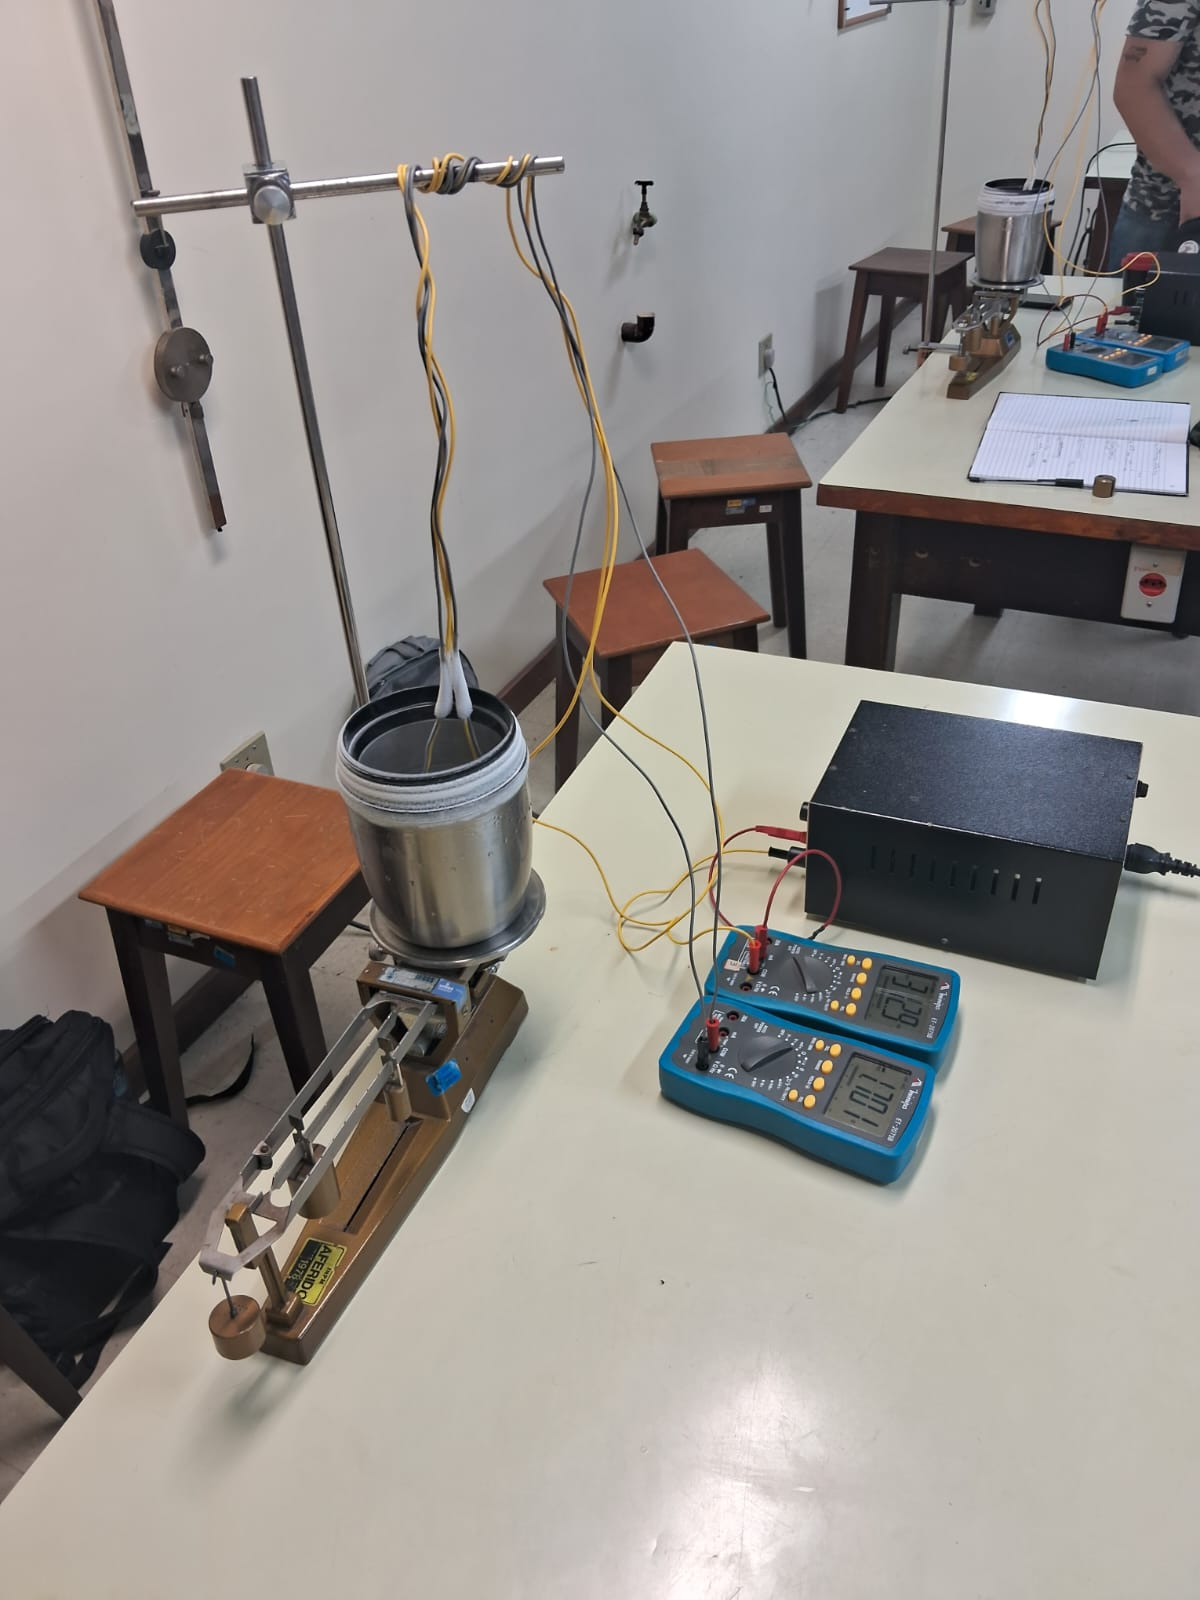
\includegraphics[width=0.45\linewidth]{montagem3.png}
    \caption{Montagem Experimental}
    \label{fig:enter-label}
\end{figure}
\section{Análise de Dados e Resultados}
\subsection*{Dados Experimentais}
O tempo encontrado para a evaporação natural foi de $245,75s$. A Tabela \ref{tab:dados} apresenta os valores de corrente, tensão, tempo e o calor latente de vaporização $L_v$ calculado para cada medida válida.

\begin{table}[!htb]
    \centering
    \caption{Dados experimentais e resultados de $L_v$}
    \label{tab:dados}
    \begin{tabular}{|c|c|c|c|c|}
        \hline
        \textbf{Medida} & \textbf{Corrente [mA]} & \textbf{Tensão [V]} & \textbf{Tempo [s]} & \textbf{$L_v$ Calculado [J/g]} \\ \hline
        1 & 201.2 & 1.100 & 238.3 & 173.97 \\ \hline
        2 & 391.9 & 2.126 & 254.44 & 111.07 \\ \hline
        3 & 311.9 & 1.696 & 220.00 & 169.55 \\ \hline
    \end{tabular}
\end{table}
\newpage
\subsection*{Resultados}
O valor experimental do calor latente de vaporização do nitrogênio líquido, considerando a média e a incerteza, calculada como desvio padrão da média, foi:
$$
    L_v = 151.5 \pm 20.3 \, \text{J/g}
$$
\begin{table}[!htb]
    \centering
    \caption{Resultados do calor latente de vaporização em diferentes unidades}
    \label{tab:conversao}
    \begin{tabular}{ |c|c|c| }
        \hline
        \textbf{Unidade} & \textbf{Valor Experimental} & \textbf{Valor Tabelado ($N_2$)} \\ \hline
        J/g & $151.5 \pm 20.3$ & 199.1 \\ \hline
        cal/g & $36.2 \pm 4.9$ & 47.6 \\ \hline
        kJ/mol & $4.24 \pm 0.57$ & 5.58 \\ \hline
    \end{tabular}
\end{table}

Comparando com o valor tabelado de $199.1 \, \text{J/g}$, o erro relativo é de $31.4\%$. Durante o experimento, enfrentamos dificuldades no sincronismo das medições de tempo e massa, o que afetou a precisão dos resultados. Medidas inconsistentes foram descartadas. Outras fontes de erro incluem variações ambientais não controladas e simplificações teóricas, como a suposição de que a potência do resistor equivale à energia transferida por calor.
\section{Conclusão}
\paragraph{}
O experimento alcançou seu objetivo de determinar o calor latente de vaporização do nitrogênio líquido, obtendo um valor experimental de $151.5\pm20.3\text{J/g}$, com um erro relativo de $31.4\%$ em relação ao valor tabelado. As principais fontes de erro incluem dificuldades no controle do sincronismo das medições de tempo e massa, variações nas condições ambientais e aproximações no modelo teórico. Apesar da discrepância, o método experimental demonstrou ser viável para estimar o calor latente de vaporização, ressaltando a importância de melhorias no controle das variáveis experimentais e na precisão das medições. Futuras repetições do experimento devem considerar mais atentamente a calibração dos instrumentos e o controle rigoroso das condições ambientais para reduzir as incertezas e aumentar a confiabilidade dos resultados.

\begin{thebibliography}{99}

\bibitem{Moyses_book}
NUSSENZVEIG, H. Moysés. {\em Curso de Física Básica - Fluidos}. 1ª ed., vol. 2. São Paulo: Edgard Blücher Ltda, 1981.

\bibitem{Laboratorio}
LIMA JUNIOR, P.; SILVA, M.T.X.; SILVEIRA, F.L.; VEIT, E.A. O laboratório de Física. Porto Alegre: IF-UFRGS, 2013. (Texto de apoio)

\bibitem{Halliday - 9 ed}
HALLIDAY, D.; RESNICK, R.; WALKER, J. {\em Fundamentos de Física}. 9ª ed. Rio de Janeiro: LTC, 2012.

\end{thebibliography}

\end{document}